
%\section{How to Use this Template}

%The template details the sections that can be used in a manuscript. Note that the order and names of article sections may differ from the requirements of the journal (e.g., the positioning of the Materials and Methods section). Please check the instructions on the authors' page of the journal to verify the correct order and names. For any questions, please contact the editorial office of the journal or support@mdpi.com. For LaTeX-related questions please contact latex@mdpi.com.
%The order of the section titles is: Introduction, Materials and Methods, Results, Discussion, Conclusions for these journals: aerospace,algorithms,antibodies,antioxidants,atmosphere,axioms,biomedicines,carbon,crystals,designs,diagnostics,environments,fermentation,fluids,forests,fractalfract,informatics,information,inventions,jfmk,jrfm,lubricants,neonatalscreening,neuroglia,particles,pharmaceutics,polymers,processes,technologies,viruses,vision

\section{Introduction}

%The introduction should briefly place the study in a broad context and highlight why it is important. It should define the purpose of the work and its significance. The current state of the research field should be reviewed carefully and key publications cited. Please highlight controversial and diverging hypotheses when necessary. Finally, briefly mention the main aim of the work and highlight the principal conclusions. As far as possible, please keep the introduction comprehensible to scientists outside your particular field of research.  %Please use the command \citep{} for the following MDPI journals, which use author--date citation: Administrative Sciences, Arts, Econometrics, Economies, Genealogy, Histories, Humanities, IJFS, Journal of Intelligence, Journalism and Media, JRFM, Languages, Laws, Religions, Risks, Social Sciences.
 
%%%%%%%%%%%%%%%%%%%%%%%%%%%%%%%%%%%%%%%%%%
\section{Materials and Methods}

%Materials and Methods should be described with sufficient details to allow others to replicate and build on published results. Please note that publication of your manuscript implicates that you must make all materials, data, computer code, and protocols associated with the publication available to readers. Please disclose at the submission stage any restrictions on the availability of materials or information. New methods and protocols should be described in detail while well-established methods can be briefly described and appropriately cited.

%Research manuscripts reporting large datasets that are deposited in a publicly avail-able database should specify where the data have been deposited and provide the relevant accession numbers. If the accession numbers have not yet been obtained at the time of submission, please state that they will be provided during review. They must be provided prior to publication.

%Interventionary studies involving animals or humans, and other studies require ethical approval must list the authority that provided approval and the corresponding ethical approval code.
%\begin{quote}
%This is an example of a quote.
%\end{quote}

\subsection{Cycle Component Modeling}

\subsubsection{Heat Exchangers}
\subsubsection{Turbines}
\subsubsection{Compressors}
\subsubsection{Concentrating Solar Power Cycle}


\subsection{Cycle Models}







%%%%%%%%%%%%%%%%%%%%%%%%%%%%%%%%%%%%%%%%%%%%%%%%%%%%%%%%%%%%%%%%%%%%%%%%%%%%%%%%%%
\section{Results}

%This section may be divided by subheadings. It should provide a concise and precise description of the experimental results, their interpretation as well as the experimental conclusions that can be drawn.

\subsection{Cycle Configurations} %========================================

\begin{specialtable}[H] 
    \caption{Constant cycle parameters with definition, variable and set value. The variables with (*) have changing labels depending on the specific cycle diagram. \label{cycle-constants}}
    \begin{tabular}{lcc}
    \toprule
    \textbf{Parameter} & \textbf{Variable}	& \textbf{Design Point Value}\\
    \midrule
    \textit{Efficiencies}\\
    Main Compressor & $\eta_{MC}$		& 0.91 (-)\\
    Re-Compressor & $\eta_{RC}$		& 0.89 (-)\\
    Turbine & $\eta_{T}$		& 0.90 (-)\\
    Pump & $\eta_{P}$      & 0.90 (-)\\
    \midrule
    \textit{Approach Temperatures}\\
    Low Temperature Recuperator & $\delta_{LTR}$		& 10 (K)\\
    High Temperature Recuperator & $\delta_{HTR}$		& 10 (K)\\
    Concentrating Solar Power Heat Exchanger & $\delta_{CSPHX}$	& 10 (K)\\
    \midrule
    \textit{Pressures}\\
    Pressure Ratio & $PR$ & 3.27 (-)\\
    High Side Pressure & (*) & 2.88e7 (Pa)\\
    \midrule
    \textit{Heat Into System}\\
    Lead-Fast Reactor Heat Transfer & $\dot{Q}_{LFRHX}$ & 9.5e8 (W)\\
    Concentrating Solar Power Heat Transfer & $\dot{Q}_{CSP}$ & 7.5e8 (W)\\
    \midrule
    \textit{Temperature}\\
    Main Compressor Inlet & (*) & 313.2 (K)\\
    Lead-Fast Reactor Low Temperature & (*) & 673.2 (K)\\
    \midrule
    \textit{Pumps}\\
    Pressure Rise Across Pump & $\Delta_{P}$ & 3.726e6 (Pa)\\
    Pump Low Side Pressure & (*) & 3.0e6 (Pa)\\ 
    \bottomrule
    \end{tabular}
\end{specialtable}

\subsubsection{C-LFR-ON} %--------------------------------------------------------
\end{paracol}
\begin{figure}[H]
    \widefigure
    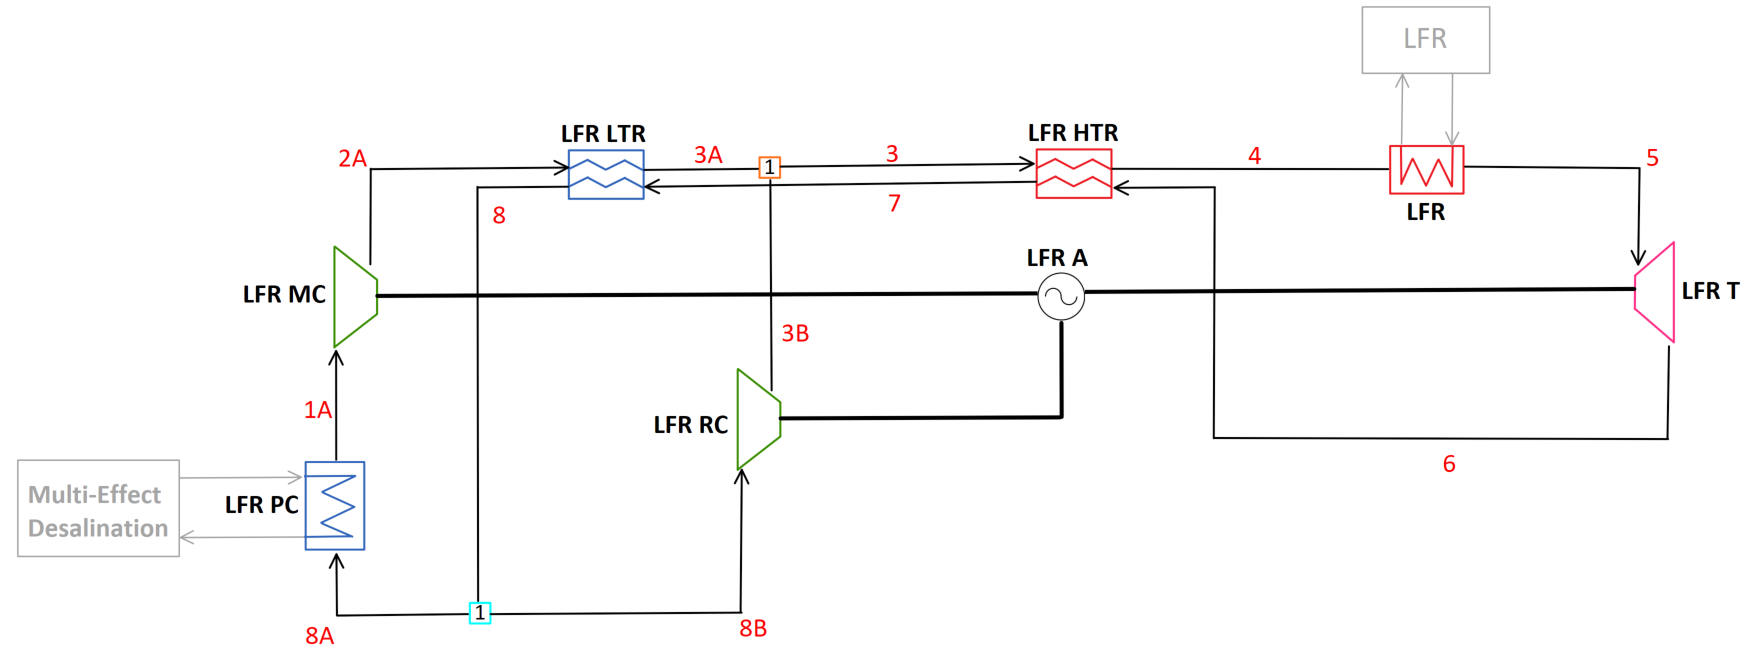
\includegraphics[width=\linewidth]{Definitions/c-lfr-on.pdf}
    \caption{Diagram for C-LFR-ON with focus on electricity generation\label{c-lfr-on}}
\end{figure}
\begin{paracol}{2}
\linenumbers
\switchcolumn

\begin{specialtable}[H] 
    \caption{State points calculated at steady state operation and LFR low temperature constrained to 673.2 K for C-LFR-ON cycle. \label{c-lfr-on-tab-cons}}
    \begin{tabular}{lcccc}
    \toprule
    \textbf{Diagram}	& \textbf{Temperature}	& \textbf{Pressure} &\textbf{Mass Flow} & \textbf{Enthalpy}\\
    \textbf{Label} & \textbf{(K)} & \textbf{(Pa)} &\textbf{(kg/s)} & \textbf{(J/kg)}\\
    \midrule
    1a-A		& 313.2  & 8.807e6  & 3029  & -149660\\
    1b-A		& 313.2  & 8.807e6  & 3029  & -149660\\
    2a-A		& 374.2  & 2.88e7  & 3029  & -110393\\
    2b-A		& 374.2  & 2.88e7  & 3029  & -110393\\
    3a-A		& 438.2  & 2.88e7  & 3029  & 10618\\
    3a-B		& 506.4  & 2.88e7  & 832.4  & 114847\\
    3b  		& 451.9  & 2.88e7  & 3861  & 33089\\
    3b-A		& 451.9  & 2.88e7  & 3861  & 33089\\
    4a-A		& 673.2  & 2.88e7  & 3861  & 333669\\
    4b  		& 673.2  & 2.88e7  & 3861  & 333669\\
    5a  		& 868.2  & 2.88e7  & 3861  & 579720\\
    5b  		& 868.2  & 2.88e7  & 3861  & 579720\\
    6a  		& 722.8  & 8.807e6  & 3861  & 417482\\
    6b  		& 722.8  & 8.807e6  & 3861  & 417482\\
    7a  		& 722.8  & 8.807e6  & 3861  & 417482\\
    7b  		& 722.8  & 8.807e6  & 3861  & 417482\\
    8a  		& 461.9  & 8.807e6  & 3861  & 116902\\
    8b  		& 461.9  & 8.807e6  & 3861  & 116902\\
    9a  		& 384.2  & 8.807e6  & 3861  & 21981\\
    9b-A		& 384.2  & 8.807e6  & 3029  & 21981\\
    9b-B		& 384.2  & 8.807e6  & 834.2  & 21981\\
    \bottomrule
    \end{tabular}
    \begin{tabular}{lcc}
    \toprule
    \textbf{Definition} & \textbf{Variable} & \textbf{Calculated Value}\\
    \midrule
    Cycle Efficiency (\%) & $\eta_{cycle}$ & 45.28\\
    Alternator Power (W) & $\dot{W}_{A}$ & 4.302e8\\
    PreCooler Heat Transfer (W) & $\dot{Q}_{PC}$ & 5.198e8\\
    Main Compressor Power (W) & $\dot{W}_{MC}$ & 1.189e8\\ 
    ReCompressor Power (W) & $\dot{W}_{RC}$ & 7.730e7\\ 
    Turbine Power (W) & $\dot{W}_{T}$ & 6.264e8\\
    Main Compressor Mass Flow Fraction (-) & $y_{1}$ & 0.7844\\
    LTR UA Value (W/K) & $UA_{LTR}$ & 2.284e7\\
    LTR Capacitance Ratio (-) & $CR_{LTR}$ & 0.8473\\
    LTR Heat Transfer Rate (W) & $\dot{Q}_{LTR}$ & 3.665e8\\
    LTR Effectiveness (-) & $\varepsilon_{LTR}$ & 0.8742\\
    HTR UA Value (W/K) & $UA_{HTR}$ & 4.271e7\\
    HTR Capacitance Ratio (-) & $CR_{HTR}$ & 0.9627\\
    HTR Heat Transfer Rate (W) & $\dot{Q}_{HTR}$ & 1.161e9\\
    HTR Effectiveness (-) & $\varepsilon_{HTR}$ & 0.9627\\
    \bottomrule
    \end{tabular}\\
\end{specialtable}

\begin{specialtable}[H] 
    \caption{State points calculated at steady state operation with LFR low temperature unconstrained and cycle efficiency maximized for C-LFR-ON cycle. \label{c-lfr-on-tab-unconst}}
    \begin{tabular}{lcccc}
    \toprule
    \textbf{Diagram}	& \textbf{Temperature}	& \textbf{Pressure} &\textbf{Mass Flow} & \textbf{Enthalpy}\\
    \textbf{Label} & \textbf{(K)} & \textbf{(Pa)} &\textbf{(kg/s)} & \textbf{(J/kg)}\\
    \midrule
    1a-A		& 313.2  & 8.807e6  & 2929  & -149660\\
    1b-A		& 313.2  & 8.807e6  & 2929  & -149660\\
    2a-A		& 374.2  & 2.88e7  & 2929  & -110393\\
    2b-A		& 374.2  & 2.88e7  & 2929  & -110393\\
    3a-A		& 505.7  & 2.88e7  & 2929  & 113832\\
    3a-B		& 506.4  & 2.88e7  & 1255  & 114847\\
    3b  		& 505.9  & 2.88e7  & 4184  & 114137\\
    3b-A		& 505.9  & 2.88e7  & 4184  & 114137\\
    4a-A		& 688.3  & 2.88e7  & 4184  & 352679\\
    4b  		& 688.3  & 2.88e7  & 4184  & 352679\\
    5a  		& 868.2  & 2.88e7  & 4184  & 579720\\
    5b  		& 868.2  & 2.88e7  & 4184  & 579720\\
    6a  		& 722.8  & 8.807e6  & 4184  & 417482\\
    6b  		& 722.8  & 8.807e6  & 4184  & 417482\\
    7a  		& 722.8  & 8.807e6  & 4184  & 417482\\
    7b  		& 722.8  & 8.807e6  & 4184  & 417482\\
    8a  		& 515.9  & 8.807e6  & 4184  & 178939\\
    8b  		& 515.9  & 8.807e6  & 4184  & 178939\\
    9a  		& 384.2  & 8.807e6  & 4184  & 21981\\
    9b-A		& 384.2  & 8.807e6  & 2929  & 21981\\
    9b-B		& 384.2  & 8.807e6  & 1255  & 21981\\
    \bottomrule
    \end{tabular}
    \begin{tabular}{lcc}
    \toprule
    \textbf{Definition} & \textbf{Variable} & \textbf{Calculated Value}\\
    \midrule
    Cycle Efficiency (\%) & $\eta_{cycle}$ & 47.08\\
    Alternator Power (W) & $\dot{W}_{A}$ & 4.473e8\\ 
    PreCooler Heat Transfer (W) & $\dot{Q}_{PC}$ & 5.027e8\\
    Main Compressor Power (W) & $\dot{W}_{MC}$ & 1.150e8\\ 
    ReCompressor Power (W) & $\dot{W}_{RC}$ & 1.166e8\\ 
    Turbine Power (W) & $\dot{W}_{T}$ & 6.789e8\\
    Main Compressor Mass Flow Fraction (-) & $y_{1}$ & 0.7000\\
    LTR UA Value (W/K) & $UA_{LTR}$ & 5.468e7\\
    LTR Capacitance Ratio (-) & $CR_{LTR}$ & 0.9867\\
    LTR Heat Transfer Rate (W) & $\dot{Q}_{LTR}$ & 6.568e8\\
    LTR Effectiveness (-) & $\varepsilon_{LTR}$ & 0.92\\
    HTR UA Value (W/K) & $UA_{HTR}$ & 4.829e7\\
    HTR Capacitance Ratio (-) & $CR_{HTR}$ & 0.8657\\
    HTR Heat Transfer Rate (W) & $\dot{Q}_{HTR}$ & 9.981e8\\
    HTR Effectiveness (-) & $\varepsilon_{HTR}$ & 0.9544\\
    \bottomrule
    \end{tabular}\\
\end{specialtable}

\subsubsection{C-CSP-ON} %--------------------------------------------------------
\end{paracol}
\begin{figure}[H]
    \widefigure
    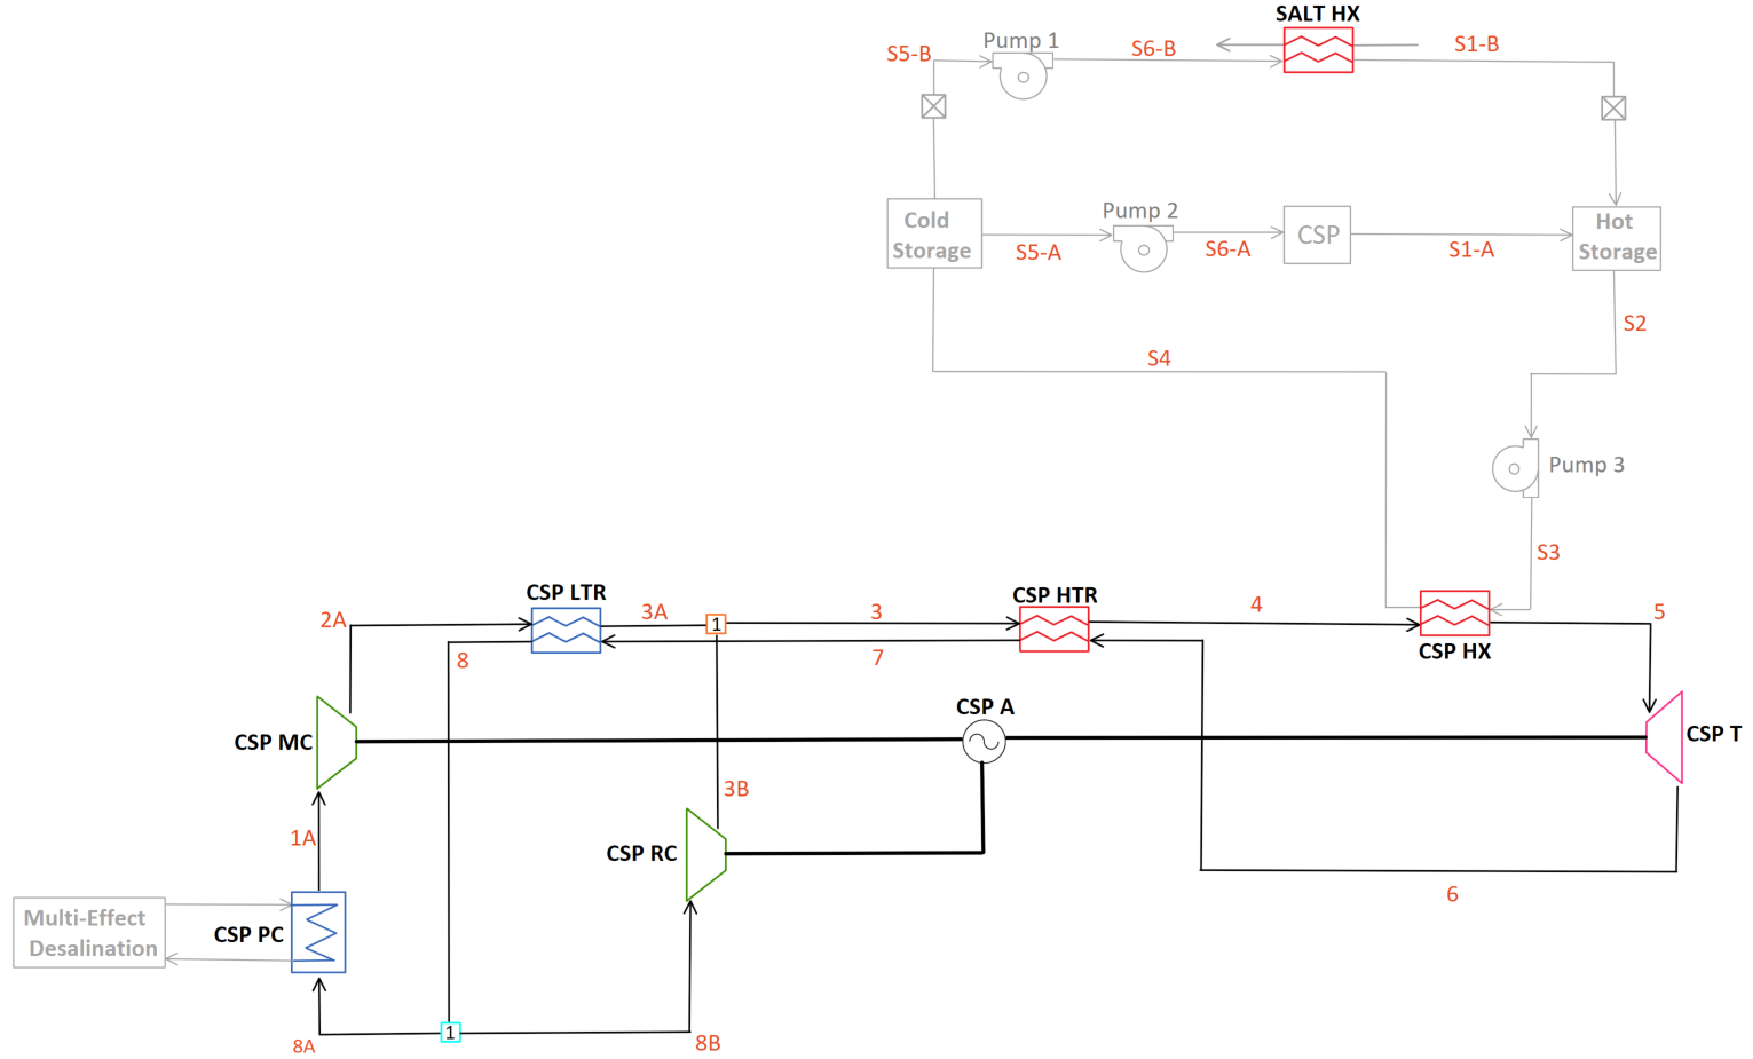
\includegraphics[width=\linewidth]{Definitions/c-csp-on.pdf}
    \caption{Diagram for C-CSP-ON with focus on electricity generation\label{c-csp-on}}
\end{figure}
\begin{paracol}{2}
\linenumbers
\switchcolumn

\subsubsection{C-1HTR1T-ON} %-----------------------------------------------------
\end{paracol}
\begin{figure}[H]
    \widefigure
    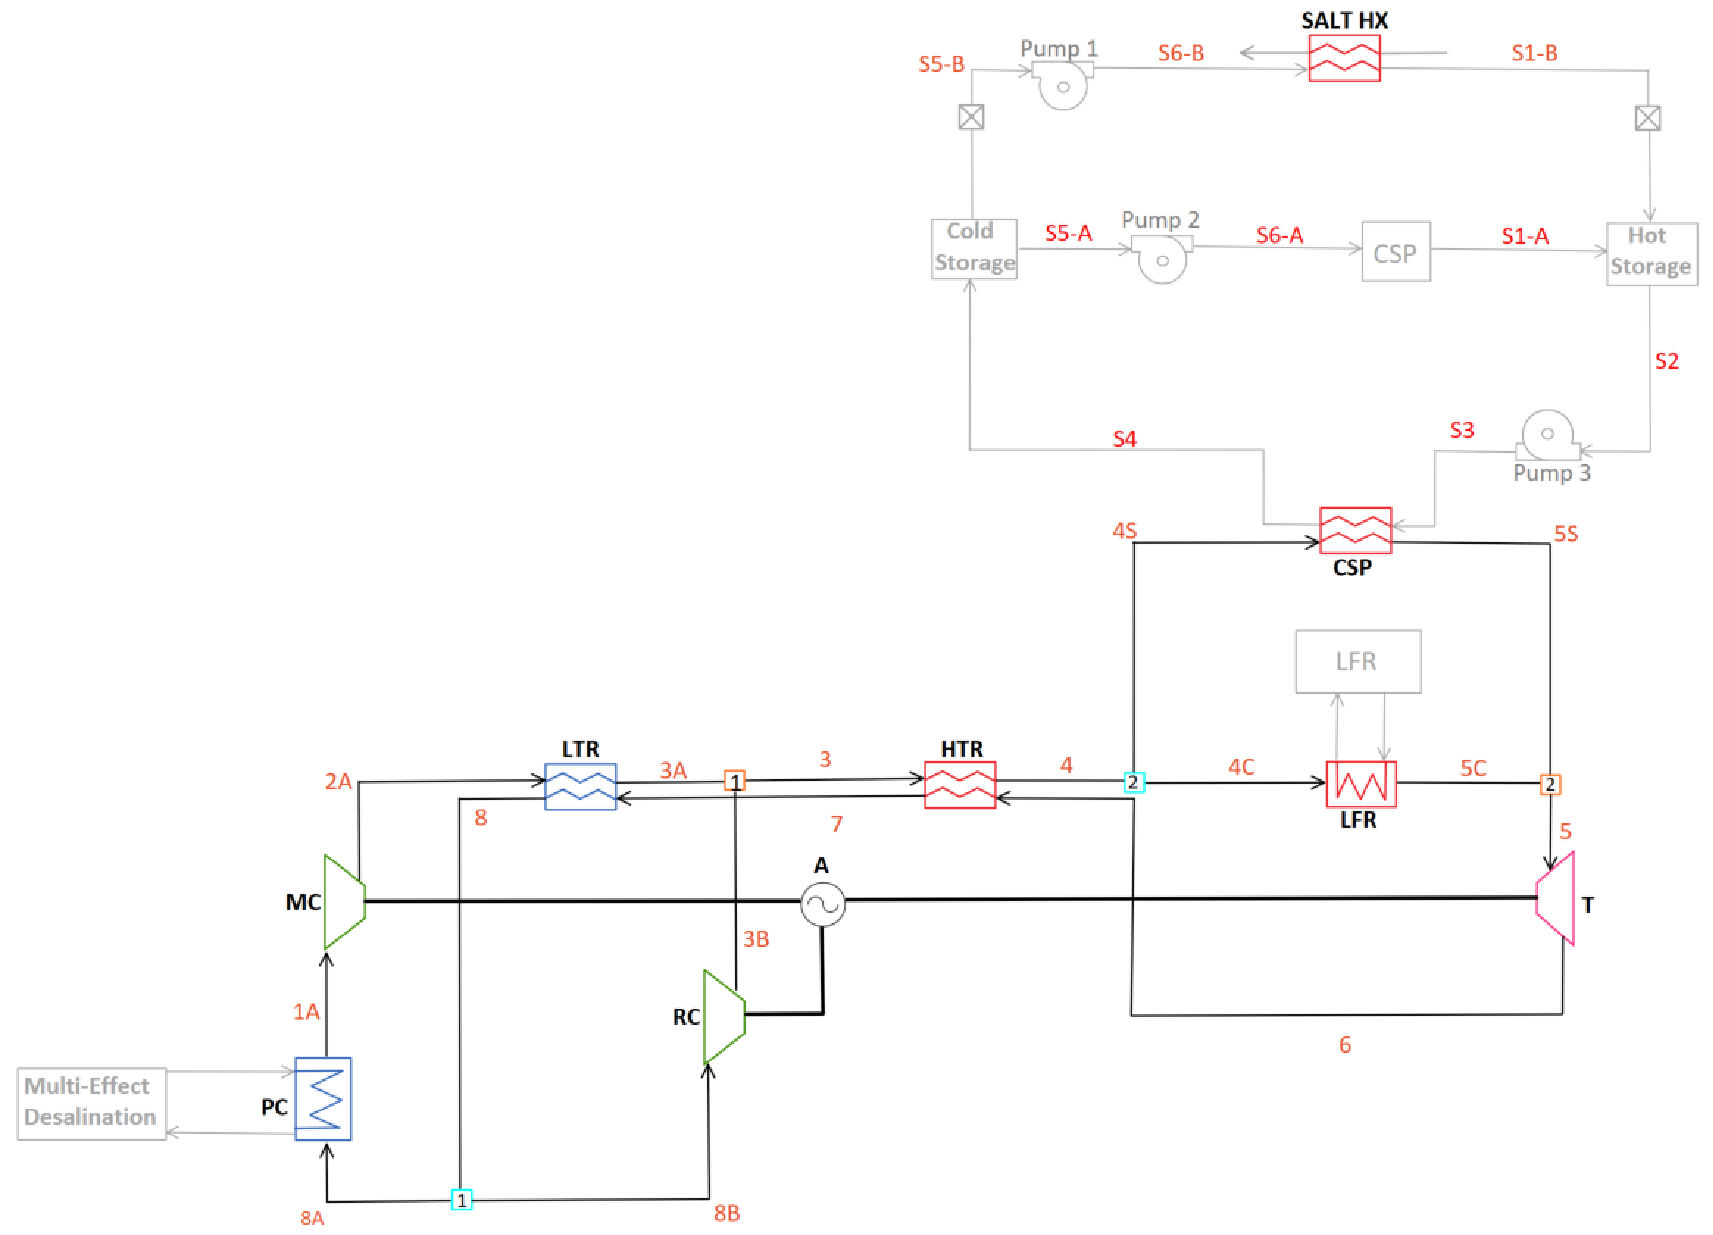
\includegraphics[width=\linewidth]{Definitions/c-1htr1t-on.pdf}
    \caption{Diagram for C-1HTR1T-ON with focus on electricity generation\label{c-1htr1t-on}}
\end{figure}
\begin{paracol}{2}
\linenumbers
\switchcolumn

\subsubsection{C-2HTR3T-ON} %-----------------------------------------------------
\end{paracol}
\begin{figure}[H]
    \widefigure
    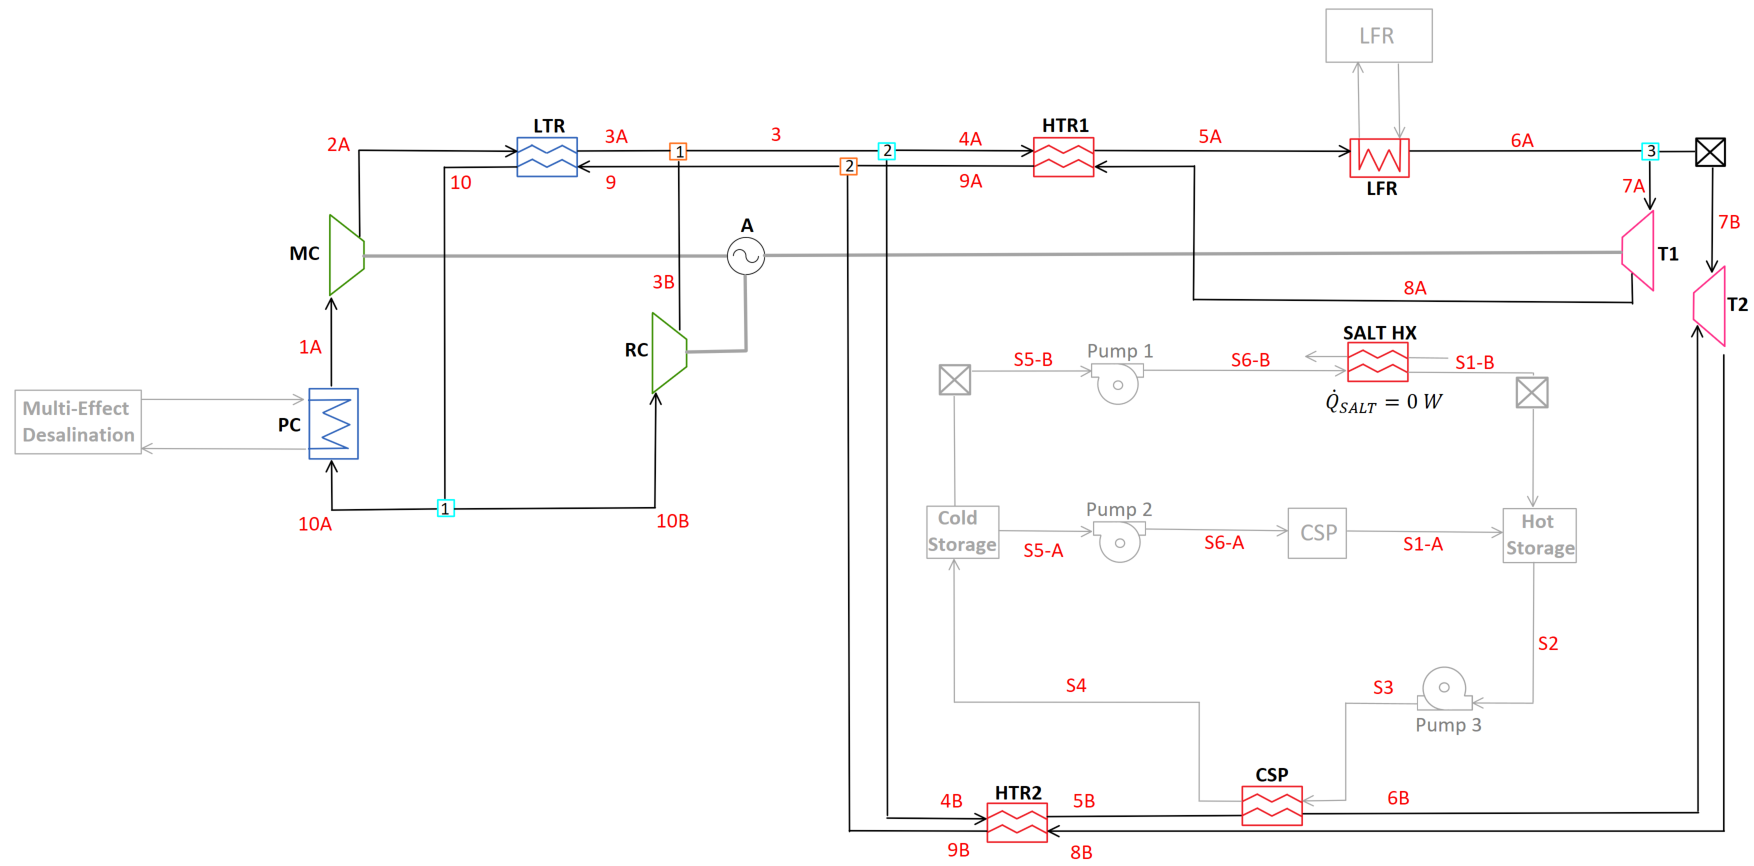
\includegraphics[width=\linewidth]{Definitions/c-2htr3t-on.pdf}
    \caption{Diagram for C-2HTR3T-ON with focus on electricity generation\label{c-2htr3t-on}}
\end{figure}
\begin{paracol}{2}
\linenumbers
\switchcolumn

\subsection{Thermal Energy Storage Charging Techniques} %=========================

\subsubsection{C-LFR-PRE} %-------------------------------------------------------
\end{paracol}
\begin{figure}[H]
    \widefigure
    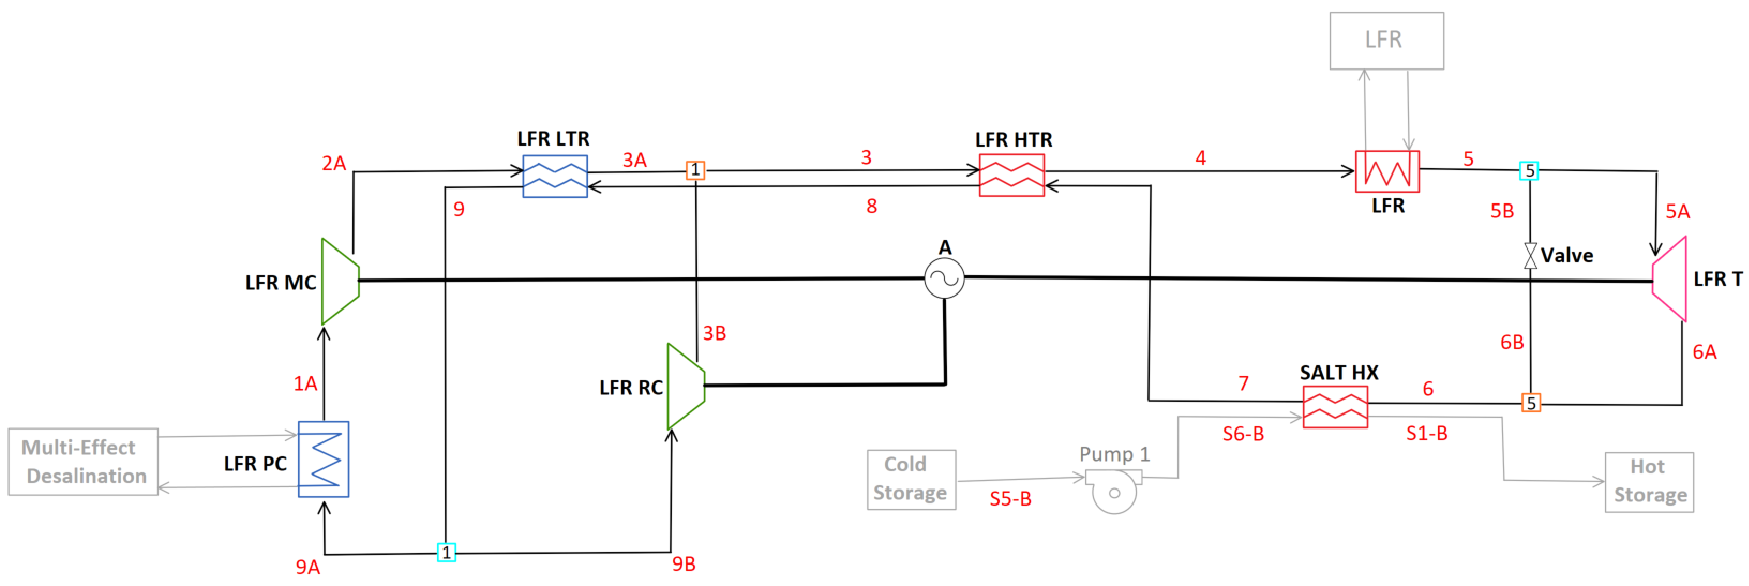
\includegraphics[width=\linewidth]{Definitions/c-lfr-pre.pdf}
    \caption{Diagram for C-LFR-PRE thermal energy storage charging orientation\label{c-lfr-pre}}
\end{figure}
\begin{paracol}{2}
\linenumbers
\switchcolumn


\subsubsection{C-LFR-POST} %------------------------------------------------------
\end{paracol}
\begin{figure}[H]
    \widefigure
    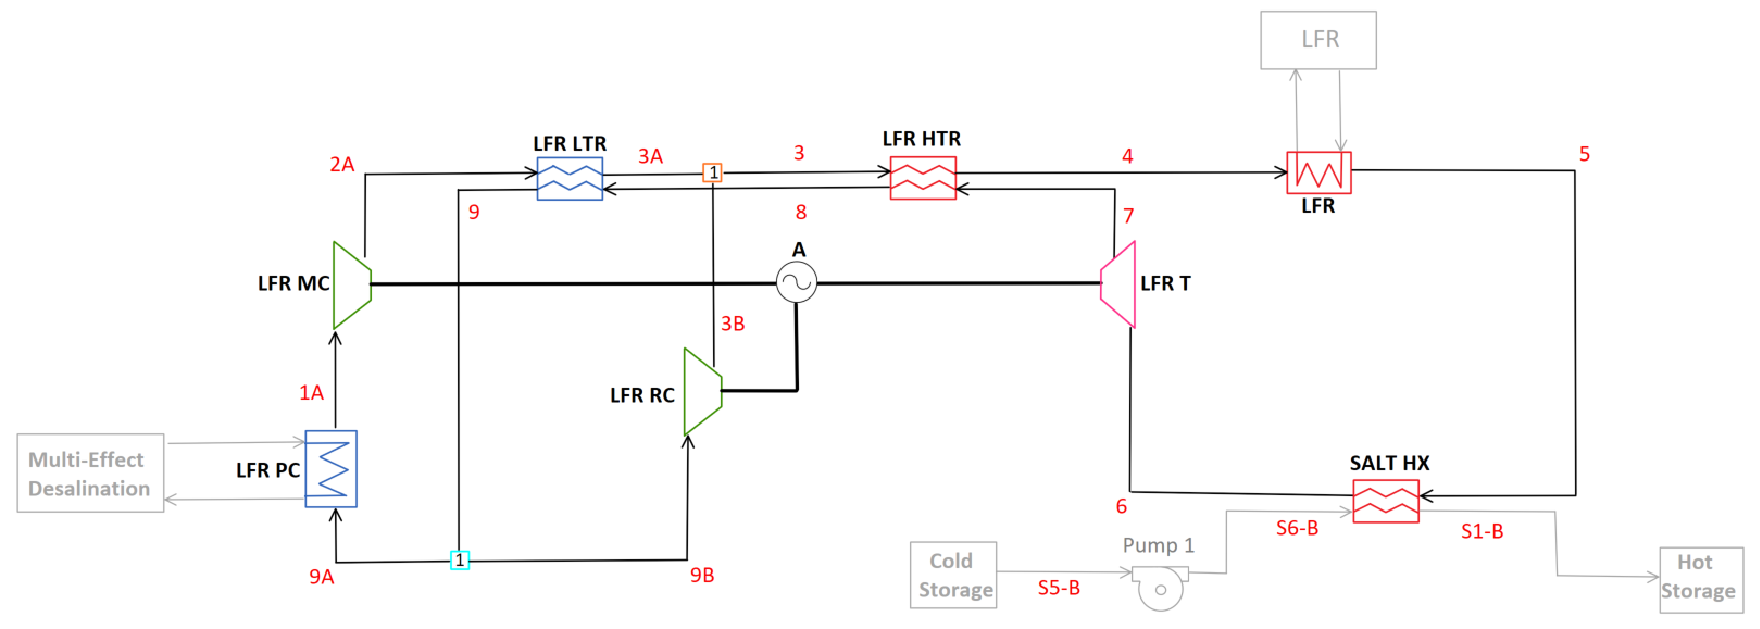
\includegraphics[width=\linewidth]{Definitions/c-lfr-post.pdf}
    \caption{Diagram for C-LFR-POST thermal energy storage charging orientation\label{c-lfr-post}}
\end{figure}
\begin{paracol}{2}
\linenumbers
\switchcolumn


\subsubsection{C-LFR-PAR} %-------------------------------------------------------
\end{paracol}
\begin{figure}[H]
    \widefigure
    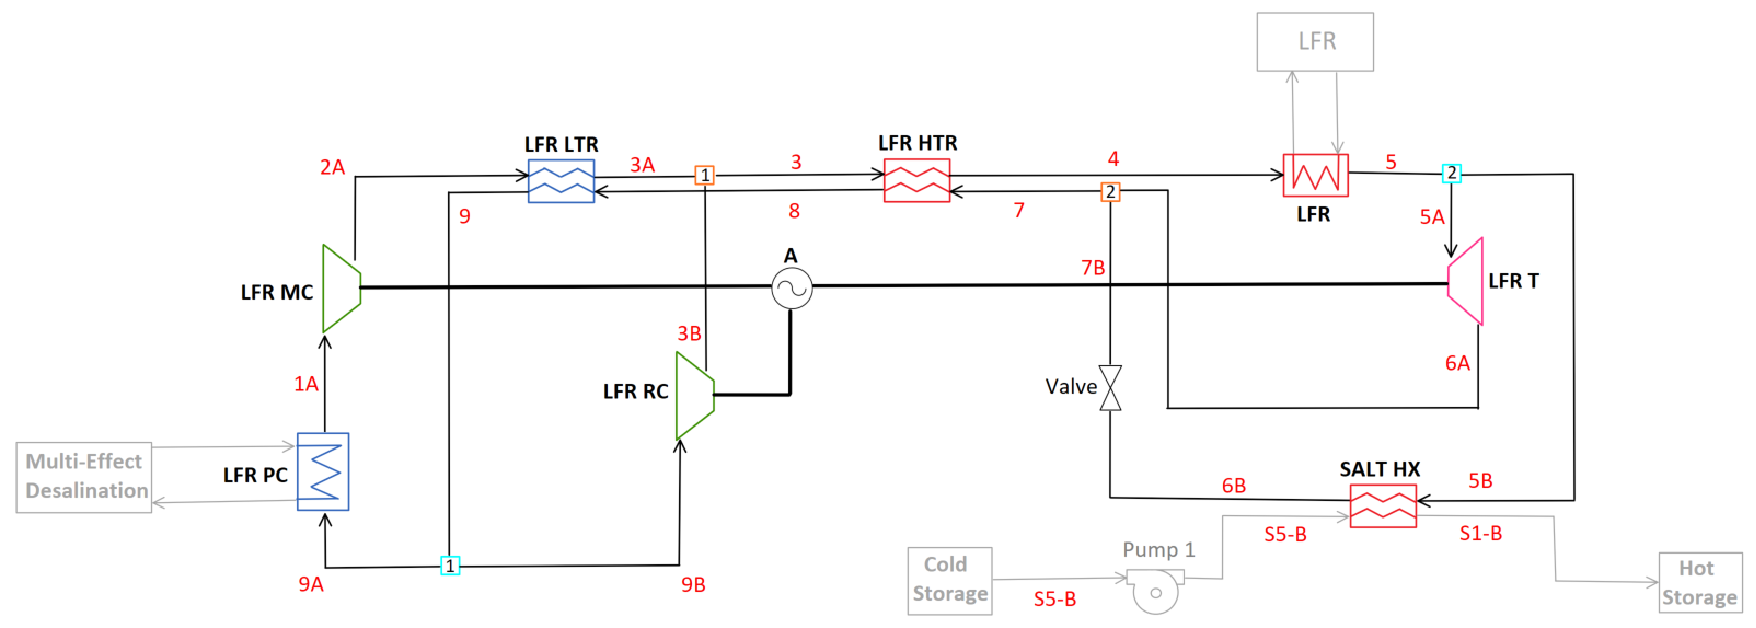
\includegraphics[width=\linewidth]{Definitions/c-lfr-par.pdf}
    \caption{Diagram for C-LFR-PAR thermal energy storage charging orientation\label{c-lfr-par}}
\end{figure}
\begin{paracol}{2}
\linenumbers
\switchcolumn

\subsubsection{C-LFR-CIRC} %------------------------------------------------------
\end{paracol}
\begin{figure}[H]
    \widefigure
    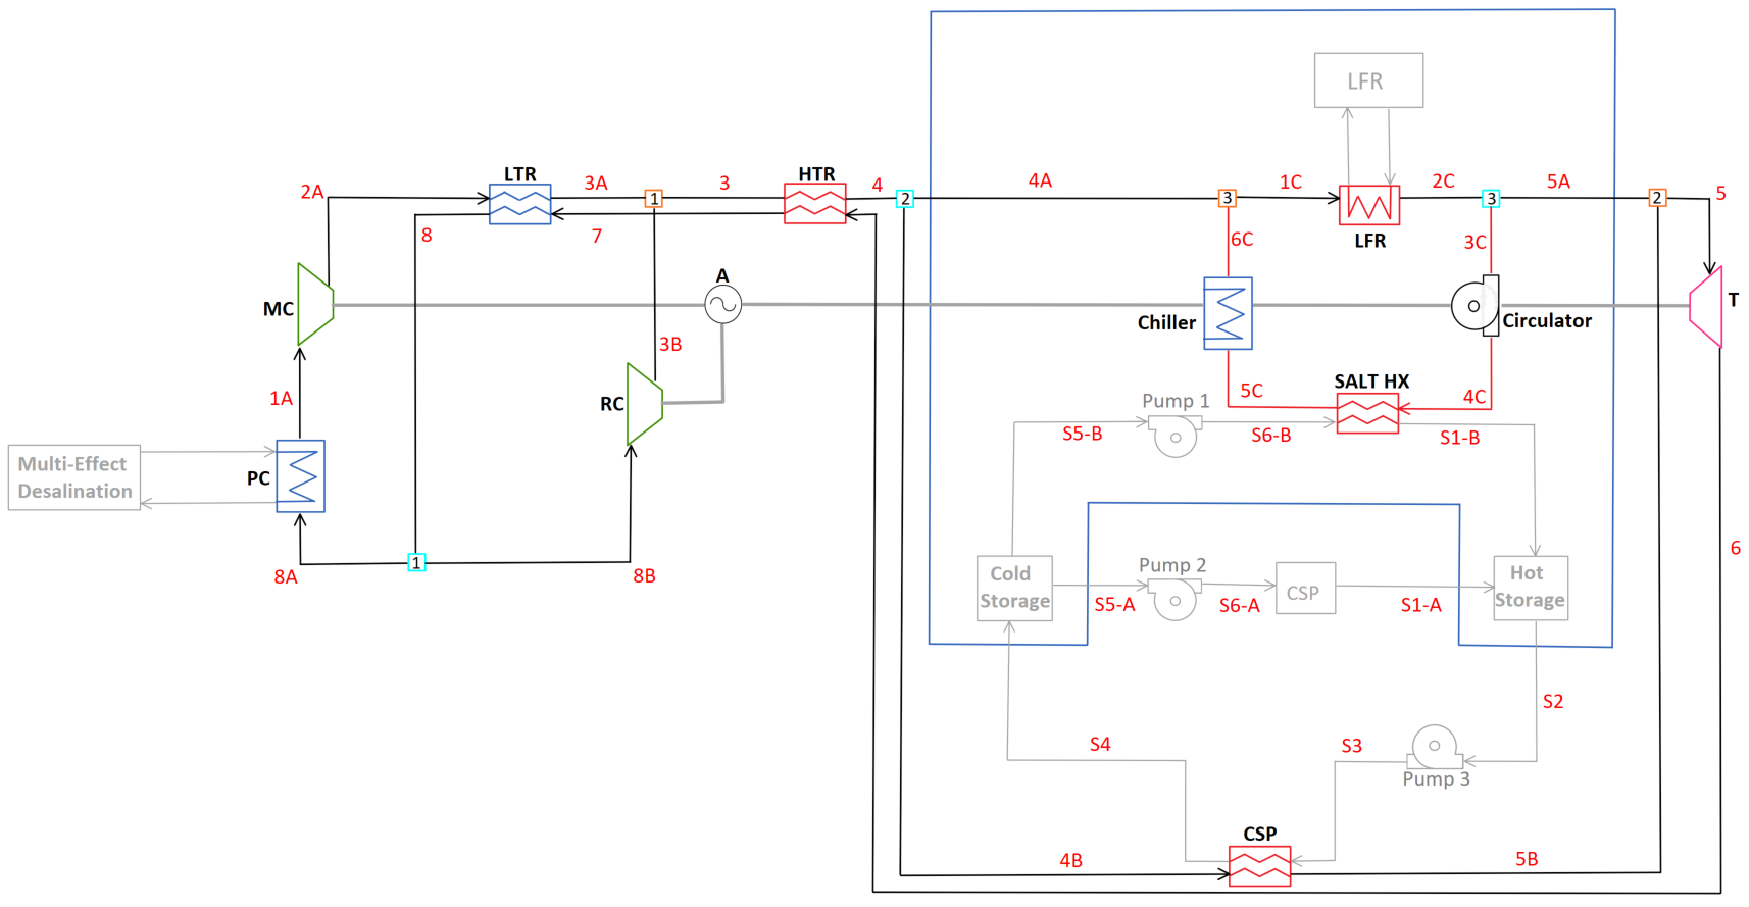
\includegraphics[width=\linewidth]{Definitions/c-lfr-circ.pdf}
    \caption{Full diagram for C-LFR-CIRC thermal energy storage charging orientation\label{c-lfr-circ}}
\end{figure}
\begin{paracol}{2}
\linenumbers
\switchcolumn

\end{paracol}
\begin{figure}[H]
    \widefigure
    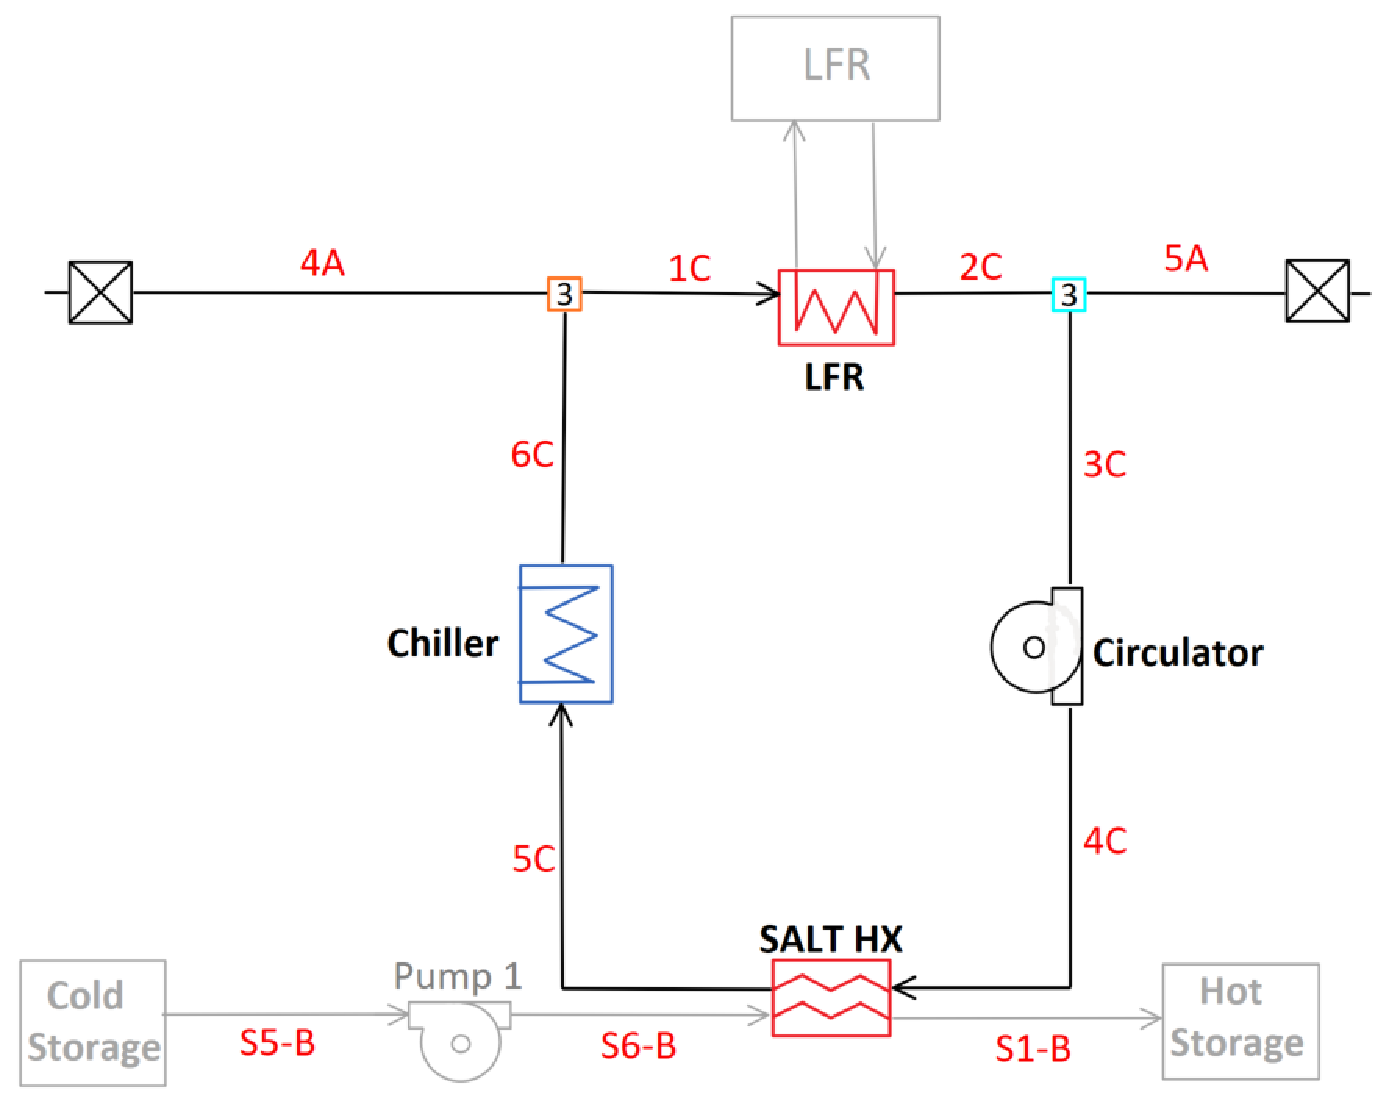
\includegraphics[width=10 cm]{Definitions/c-lfr-circ-sub.pdf}
    \caption{Diagram for C-LFR-CIRC subcycle thermal energy storage charging orientation\label{c-lfr-circ-sub}}
\end{figure}
\begin{paracol}{2}
\linenumbers
\switchcolumn





%%%%%%%%%%%%%%%%%%%%%%%%%%%%%%%%%%%%%%%%%%
\section{Discussion}

Authors should discuss the results and how they can be interpreted from the perspective of previous studies and of the working hypotheses. The findings and their implications should be discussed in the broadest context possible. Future research directions may also be highlighted.

%%%%%%%%%%%%%%%%%%%%%%%%%%%%%%%%%%%%%%%%%%
\section{Conclusions}

This section is not mandatory, but can be added to the manuscript if the discussion is unusually long or complex.

%%%%%%%%%%%%%%%%%%%%%%%%%%%%%%%%%%%%%%%%%%
\section{how to use}

\subsection{Subsection}
Citing a journal paper \cite{wagner2017optimization} . Now citing a book reference \cite{blair2005sam} or other reference types \cite{hirsch2011standardization}. \cite{nellis_klein_2008}
\subsubsection{Subsubsection}

Bulleted lists look like this:
\begin{itemize}
\item	First bullet;
\item	Second bullet;
\item	Third bullet.
\end{itemize}

Numbered lists can be added as follows:
\begin{enumerate}
\item	First item; 
\item	Second item;
\item	Third item.
\end{enumerate}

The text continues here. 

\subsection{Figures, Tables and Schemes}

All figures and tables should be cited in the main text as Figure~\ref{fig1}, Table~\ref{tab1}, etc.

\begin{figure}[H]

\includegraphics[width=10.5 cm]{Definitions/logo-mdpi}
\caption{This is a figure. Schemes follow the same formatting. If there are multiple panels, they should be listed as: (\textbf{a}) Description of what is contained in the first panel. (\textbf{b}) Description of what is contained in the second panel. Figures should be placed in the main text near to the first time they are cited. A caption on a single line should be centered.\label{fig1}}
\end{figure}   

% The MDPI table float is called specialtable
\begin{specialtable}[H] 
\caption{This is a table caption. Tables should be placed in the main text near to the first time they are~cited.\label{tab1}}
%%% \tablesize{} %% You can specify the fontsize here, e.g., \tablesize{\footnotesize}. If commented out \small will be used.
\begin{tabular}{ccc}
\toprule
\textbf{Title 1}	& \textbf{Title 2}	& \textbf{Title 3}\\
\midrule
Entry 1		& Data			& Data\\
Entry 2		& Data			& Data\\
\bottomrule
\end{tabular}
\end{specialtable}

%\begin{listing}[H]
%\caption{Title of the listing}
%\rule{\columnwidth}{1pt}
%\raggedright Text of the listing. In font size footnotesize, small, or normalsize. Preferred format: left aligned and single spaced. Preferred border format: top border line and bottom border line.
%\rule{\columnwidth}{1pt}
%\end{listing}

Text.

Text.

\subsection{Formatting of Mathematical Components}

This is the example 1 of equation:
\begin{equation}
a = 1,
\end{equation}
the text following an equation need not be a new paragraph. Please punctuate equations as regular text.
%% If the documentclass option "submit" is chosen, please insert a blank line before and after any math environment (equation and eqnarray environments). This ensures correct linenumbering. The blank line should be removed when the documentclass option is changed to "accept" because the text following an equation should not be a new paragraph.

This is the example 2 of equation:
\end{paracol}
\nointerlineskip
\begin{eqnarray}
a &=& b + c + d + e + f + g + h + i + j + k + l\nonumber \\
 &+& m + n + o + p + q + r + s + t + u + v + w + x + y + z %\nonumber
\end{eqnarray}

% Example of a figure that spans the whole page width (the commands \widefigure and \begin{paracol}{2}, \linenumbers, and\switchcolumn need to be present). The same concept works for tables, too.
%\begin{figure}[H]	
%\widefigure
%
\includegraphics[width=15 cm]{Definitions/logo-mdpi}
%\caption{This is a wide figure.\label{fig2}}
%\end{figure} 





\begin{paracol}{2}
\linenumbers
\switchcolumn
Please punctuate equations as regular text. Theorem-type environments (including propositions, lemmas, corollaries etc.) can be formatted as follows:
%% Example of a theorem:
\begin{Theorem}
Example text of a theorem.
\end{Theorem}

The text continues here. Proofs must be formatted as follows:

%% Example of a proof:
\begin{proof}[Proof of Theorem 1]
Text of the proof. Note that the phrase ``of Theorem 1'' is optional if it is clear which theorem is being referred to.
\end{proof}
The text continues here.

\end{paracol}
